\documentclass[
  captions=tableheading,
  bibliography=totoc, 
  titepage=firstiscover,
]{scrartcl}

\usepackage{blindtext} %neuer input

\usepackage{longtable} % Tabellen über mehrere Seiten

\usepackage[utf8]{inputenc} %neuer input

\usepackage{scrhack}

\usepackage[aux]{rerunfilecheck} %Warnung falls nochmal kompiliert werden muss

\usepackage{fontspec} %Fonteinstellungen

\recalctypearea{}

\usepackage[main=ngerman]{babel} %deutsche Spracheinstellung

\usepackage{ragged2e} %neuer input

\usepackage{amsmath, nccmath}

\usepackage{amssymb} %viele mathe Symbole

\usepackage{mathtools} %Erweiterungen für amsmath


\DeclarePairedDelimiter{\abs}{\lvert}{\rvert}
\DeclarePairedDelimiter{\norm}{\lVert}{\rVert}

\DeclarePairedDelimiter{\bra}{\langle}{\rvert}
\DeclarePairedDelimiter{\ket}{\lvert}{\rangle}

\DeclarePairedDelimiterX{\braket}[2]{\langle}{\rangle}{
#1 \delimsize| #2
}

\NewDocumentCommand \dif {m}
{
\mathinner{\symup{d} #1}
}


\usepackage[
  math-style=ISO,
  bold-style=ISO,
  sans-style=italic,
  nabla=upright,
  partial=upright,
  warnings-off={
    mathtools-colon,
    mathtools-overbracket,
  },
]{unicode-math}

\setmathfont{Latin Modern Math}
\setmathfont{XITS Math}[range={scr, bfscr}]
\setmathfont{XITS Math}[range={cal, bfcal}, StylisticSet=1]


\usepackage[
  locale=DE,
  separate-uncertainty=true,
  per-mode=reciprocal,
  output-decimal-marker={,},
]{siunitx}

\usepackage[autostyle]{csquotes} %richtige Anführungszeichen

\usepackage{xfrac}

\usepackage{float}

\floatplacement{figure}{htbp}

\floatplacement{table}{htbp}

\usepackage[ %floats innerhalb einer section halten
  section,   %floats innerhalb er section halten
  below,     %unterhalb der Section aber auf der selben Seite ist ok
]{placeins}

\usepackage[
  labelfont=bf,
  font=small,
  width=0.9\textwidth,
]{caption}

\usepackage{subcaption} %subfigure, subtable, subref

\usepackage{graphicx}

\usepackage{grffile}

\usepackage{booktabs}

\usepackage{microtype} %Verbesserungen am Schriftbild

\usepackage[
backend=biber,
]{biblatex}

\addbibresource{../lit.bib}

\usepackage[ %Hyperlinks im Dokument
  german,
  unicode,
  pdfusetitle,
  pdfcreator={},
  pdfproducer={},
]{hyperref}

\usepackage{bookmark}

\usepackage[shortcuts]{extdash}

%\usepackage{warpcol}


\begin{document}
    \title{V103 Biegung elastischer Stäbe}
    \author{  
    Tobias Rücker\\
    \texorpdfstring{\href{mailto:tobias.ruecker@tu-dortmund.de}{tobias.ruecker@tu-dortmund.de}
    \and}{,} 
    Paul Störbrock\\
    \texorpdfstring{\href{mailto:paul.stoerbrock@tu-dortmund.de}{paul.stoerbrock@tu-dortmund.de}}{}
    }
    \date{Durchführung: 10.12.2019, Abgabe: 17.12.2019\vspace{-4ex}}
\maketitle
\center{\Large Versuchsgruppe: \textbf{42}}

\newpage
\tableofcontents
\newpage

% Theorie %%%%%%%%%%%%%%%%%%%%%%%%%%%%%%%%%%%%%%%%%%%%%%%%%%%%%%%%%%%%%%%%%%%%%%%%%%%%%%%%%%%%%%%%%%%%%%%%%
\section{Ziel}\justifying
Die Eigenschaften von Werkstoffen bilden in der heutigen Wissenschaft und Industrie ein Grundwissen, um 
für gegebene Probleme die optimalen Materialien zu finden. Eine Eigenschaft, die unteranderem im Bau von
Kränen oder Windkraftwerken relevant ist, 
bildet der Elastizitätsmodul. Daher werden im folgenden der Elastizitätsmodul von zwei metallischen
Stäben anhand einer einseitig und doppeltseitig fixierten Biegung bestimmt.

\section{Theorie}\label{sec:1}\justifying
Ein Körper erfährt eine Volumenänderung, wenn an dessen Oberfläche eine Kraft angelegt
wird. Diese Kraft hat einen engen Bezug zur Fläche des Körpers und wird in der Physik
als Spannung $\sigma$ bezeichnet.\\
Ein Beispiel für eine Volumenveränderung stellt die einseitige Biegung eines Stabes dar.
Dabei wird ein Ende des Stabes fixiert, während auf dem anderen Ende des Stabes eine
Gewichtskraft über eine zusätzliche Masse wirkt. Dadurch wird das fixierte Ende des Stabes gestreckt,
das Mittelstück des Stabes gestaucht und das Ende mit der Masse bleibt gleich. Der Stab stellt dabei aufgrund der inneren
Kräfte und der elastischen Eigenschaften eine konstante Auslenkung ein.
Bei kleinen Veränderungen
besteht ein linearer Zusammenhang zwischen der Spannung $\sigma$  und der Deformation $\sfrac{\delta x}{\Delta x} $.
Dabei stimmen die Drehmomente der äußeren Kraft mit dem Drehmoment der inneren Zug- und Druckspannungen
überein. Dadurch wird die Spannung $\sigma(y)$ zu \cite{V103}
\begin{align}
    \sigma (y)=E \frac{\delta x}{\Delta x} \label{eq:1}.
\end{align}
Diese Kraft wird auch das Hooksche Gesetz genannt. Der Faktor E in der Formel wird
der Elastizitätmodul genannt und stellt eine Materialkonstante dar.
Das durch die Biegung beschriebene Drehmoment führt nach einer Kleinwinkelnäherung zu folgender Momentengleichung \cite{V103}
\begin{align}
    E \frac{\symup{d}^2 \, D}{\symup{d}x^2}\int_Q y^2 \, \symup{d}q = F(L-x) .\label{eq:2}
\end{align}
Dabei ist D die Durchbiegung des Stabes, L die Länge des Stabes beginnend an dem Fixpunkt, $F(L-x)$ der Betrag des Drehmoments und \cite{V103}
\begin{align}
    I := \int_Q y^2 \, \symup{d}q(y) \label{eq:3}
\end{align}
das Flächenträgheitsmoment. \\
Aus Gleichung \eqref{eq:2} folgt für die Durchbiegung D \cite{V103}
\begin{align}
    D(x)=\frac{F}{2E\,I}\left(L  x^2-\frac{x^3}{3}\right) \label{eq:4} (\text{für} \, 0\leq x \leq L).
\end{align}
Eine weitere mögliche Biegungsart stellt die beidseitig fixierte Biegung dar. Bei dieser wird
der Stab an beiden Enden aufgelegt und die Gewichte werden an die Stabmitte 
gehangen. \\
Für die Beschreibung der Durchbiegung wird in diesem Fall zwischen den Bereichen
$ 0\leq x\leq \sfrac{L}{2} $ und $\sfrac{L}{2} \leq x \leq L $ unterschieden.\\
Für den Bereich $0\leq x\leq \sfrac{L}{2}$ ergibt sich für D \cite{V103}
\begin{align}
    D(x)=\frac{F}{48\, E\, I}(3L^2x-4x^3) \label{eq:5}
\end{align}
und für den anderen Bereich $\sfrac{L}{2} \leq x \leq L $ ergibt sich entsprechend \cite{V103}
\begin{align}
    D(x)=\frac{F}{48\, E\, I}(4x^3 - 12Lx^2 +9L^2x-L^3) \label{eq:6}.
\end{align}
Bei der Doppelbiegung stellt L den Abstand der Auflagepunkte voneinander dar.

% Fehlerrechnung %%%%%%%%%%%%%%%%%%%%%%%%%%%%%%%%%%%%%%%%%%%%%%%%%%%%%%%%%%%%%%%%%%%%%%%%%%%%%%%%%%%%%%%%%%%%%%%%%%%

\section{Fehlerrechnung}\justifying
Für eventuell anfallende Fehler in der Auswertung werden folgende Formeln verwendet:
\begin{subequations}
\begin{align}
\intertext{Für den Mittelwert wird die Formel
}
    \overline{x} &= \frac{1}{N}\sum_{i=1}^{N} x_i \label{eq:7a}
\intertext{verwendet. Der Fehler des Mittelwerts wird mit der Formel
}
    \Delta\overline{x} &= \frac{1}{\sqrt{N}} \sqrt{\frac{1}{1-N} \sum_{i=1}^{N} (x_i - \overline{x})^2} \label{eq:7b},
\intertext{berechnet, und die Gaußsche Fehlerfortpflanzung wird wie folgt bestimmt:
}
    \Delta f &= \sqrt{\sum_{i=1}^{N} \left( \frac{\delta f}{\delta x_i} \right)^2 \cdot (\Delta x_i)^2} \label{eq:7c}
\intertext{Die für eine lineare Regression benötigte Ausgleichsgerade wird mit den folgenden Parametern berechnet:
}
    y &= m \cdot x + b \label{eq:7d} \\ 
    m &= \frac{\overline{xy} - \overline{x} \cdot \overline{y}}{\overline{x^2} - {\overline{x}}^2} \label{eq:7e}\\
    b &= \frac{\overline{y} \cdot \overline{x^2} - \overline{xy} \cdot \overline{x}}{\overline{x^2} - {\overline{x}}^2} \label{eq:7f}
\end{align}
\end{subequations}
\newpage

% Versuchsaufbau/Versuchsdurchführung %%%%%%%%%%%%%%%%%%%%%%%%%%%%%%%%%%%%%%%%%%%%%%%%%%%%%%%%%%%%%%%%%%%%%%%%%%%%%%%%%%%%%%%%%%%%%%%%%%%%%%%%%%%%%%%%%%%%%%%%%%%%%%%%%%%%%%%%%%%%%%%%%%%%%%

\section{Versuchsaufbau/Durchführung}\justifying

\flushleft{Benötigt\;}\justifying werden: \textit{ Eine ca. $\SI{60}{\centi\meter}$ lange, $\SI{530}{\gram}$ schwere, rechtreckige Metallstange, eine ca. $\SI{60}{\centi\meter}$ lange, runde
Metallstange, eine Apperatur zur Biegung der Stäbe mit zwei Fixpunkten, zwei schiebbare Messuhren im $\SI{}{\micro\meter}$-Bereich, eine
$\SI{55}{\centi\meter}$ lange Skala für die Messuhren, eine Aufhängung ($\SI{19}{\gram}$), acht Gewichte ($4\times$ ca. $\SI{1160}{\gram}$, 
$2\times$ ca. $\SI{500}{\gram}$, $1\times$ ca. $\SI{225}{\gram}$), eine Bindung für die Gewichte (hier eine Schraube ($\SI{22.1}{\gram}$))
ein Maßband, eine Waage.
}

\flushleft{Zuerst\;}\justifying wird die Aperatur wie in der folgenden Abbildung \ref{fig:aufb} aufgebaut. 

\begin{figure}
    \centering
    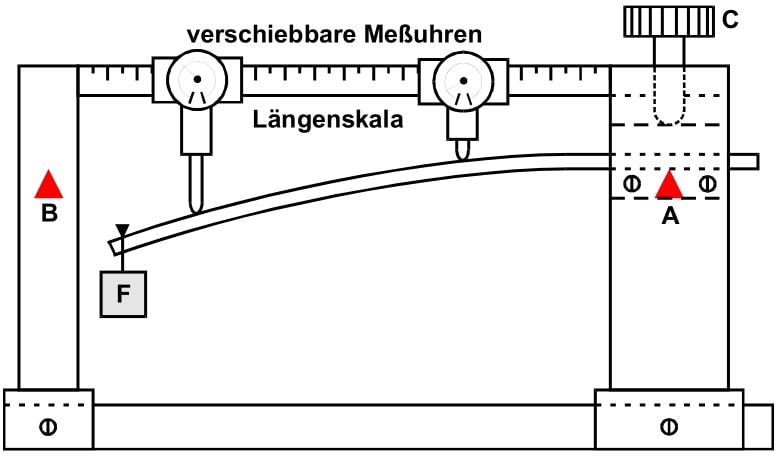
\includegraphics[width=0.75\linewidth]{./images/Aufbau_V103.jpg}
    \caption{Aufbau der einseitigen Biegung \cite{V103}}
    \label{fig:aufb}
\end{figure}

\flushleft{Anschließend\;}\justifying wird die eckige Stange an dem Skalennullpunkt eingespannt. Die Messuhren werden über der Stange auf der Skala platziert. Nun werden mit 
einer Messuhr 19 Messwerte der Durchbiegung in einem Abstand von $\SI{2.5}{\centi\meter}$ (von $\SI{2.5}{\centi\meter}$ bis $\SI{47.5}{\centi\meter}$) 
bestimmt. Nach den Messungen ohne Gewicht, werden zwei Gewichte an das lose Ende gehangen und die Messungen wiederholt. Anschließend
werden die Gewichte abgenommen und die eckige Stange an beiden Enden fixiert. Dabei ist zu beachten, dass beide Enden lose eingespannt werden, sodass die
Stange nur auf den Fixpunkten aufliegt. Nun wird die Durchbiegung an 14 Stellen mit einem Abstand von $\SI{3}{\centi\meter}$ gemessen. Danach werden vier 
Gewichte mittig an die Stange gehangen und die Messungen wiederholt. Anschließend werden die Länge und Breite des Stabs an zehn 
verschiedenen Stellen gemessen.

\flushleft{Der\;}\justifying obige Prozess wird für die runde Stange wiederholt. Zu Beginn wird die Stange einseitig eingespannt. Die Durchbiegung
wird ohne Gewichte 19-mal in einem Abstand von $\SI{2.5}{\centi\meter}$ gemessen. Dann wird ein Gewicht an das lose Ende 
gehangen und die Messung wiederholt. Anschließend wird das Gewicht abgenommen und die Stange an beiden Seiten fixiert. Auch hier dürfen die beiden Enden
nicht fest eingespannt werden. Abschließend werden 14 Messungen ohne Gewichte und 14 Messungen mit drei Gewichten durchgeführt. Wie bei der eckigen Stange
wird auch hier der Durchmesser an zehn verschiedenen Stellen des Stabs abgenommen.

% Auswertung %%%%%%%%%%%%%%%%%%%%%%%%%%%%%%%%%%%%%%%%%%%%%%%%%%%%%%%%%%%%%%%%%%%%%%%%%%%%%%%%%%%%%%%%%%%%%%%%%%%%%%%%%%%%%%%%%%%%%%%%%%%%%%%%%%%%%%%%%%%

\section{Auswertung}\justifying

% Cu_ein --------------------------------------------------------------------------------------------------------------------------------

\subsection{Kupfer einfach fixiert}\label{sec:4.1}

\flushleft{Es\;}\justifying handelt sich bei der Eckigen Stange um Kupfer, da das Material auf den Stab geschrieben wurde. 
Wird die Dichte mit den folgenden Werten \eqref{eq:8a}, \eqref{eq:8b} und \eqref{eq:8c} und der Formel $\rho = \sfrac{m}{V}$
berechnet, ergibt sich $\rho = \SI{8.864}{\gram\per\cubic\centi\meter}$. Wird dieser Wert mit dem Literaturwert der Kupferdichte
$\rho = \SI{8.9}{\gram\per\cubic\centi\meter}$ \cite{Kupferdichte} verglichen, wird die Stabaufschrift bestätigt und es handelt sich 
hierbei wahrscheinlich um Kupfer.
Die Maße und das Gewicht des Kupferstabs, sowie die Gewichte der Aufhängung und Schraube, an welche die Gewichte gehangen 
werden, sind im Folgenden aufgelistet: 
\begin{subequations}\label{eq:8}
\begin{align}
    &\text{Länge des Kupferstabs:} \qquad &\text{\input{l_Cu.tex}} \label{eq:8a}\\
    &\text{Mittelwert der Breite des Kupferstabs $\overline{b}$:} \qquad &\text{\input{d_Cu.tex}} \label{eq:8b}\\
    &\text{Mittelwert der Dicke des Kupferstabs $\overline{d}$:} \qquad &\text{\input{b_Cu.tex}} \label{eq:8c}\\
    &\text{Masse der Aufhängung:} \qquad &\text{\input{m_aufhaeng.tex}} \label{eq:8d}\\
    &\text{Masse der Schraube:} \qquad &\text{\input{m_schraube.tex}} \label{eq:8e}
\end{align}
\end{subequations}

\begin{table}[H]
\centering
    \begin{tabular}{c c c c}
    \toprule
        {$b \:/\: \si{\milli\meter}$} & {$d \:/\: \si{\milli\meter}$} & {$b \:/\: \si{\milli\meter}$} & {$d \:/\: \si{\milli\meter}$}\\
        \cmidrule(lr{0,5em}){1-2} \cmidrule(lr{0,5em}){3-4}
        10.06 & 10.02 & 10.03 & 10.09\\
        10.02 & 10.05 & 10.04 & 10.04\\
        10.05 & 10.06 & 10.02 & 10.05\\
        10.01 & 10.03 & 10.04 & 10.08\\
        10.03 & 10.04 & 10.03 & 10.05\\
    \bottomrule
    \end{tabular}
\caption{Messwerte der Breite und Dicke des Kupferstabs}
\label{tab:1}
\end{table}

\flushleft{Die\;}\justifying Mittelwerte für die Dicke $\overline{d}$ und die Breite $\overline{b}$ wurden im Folgenden mit Tabelle \ref{tab:1} 
 und Formel \eqref{eq:7a} berechnet. Um das Flächenträgheitsmoment eines rechteckigen Stabes mit der Breite b und der
Dicke d zu berechnen, welcher in z-Richtung gebogen wird, wird die Formel \eqref{eq:3} auf folgende Art
geschrieben:
\begin{align}
    I=\int_{-\frac{b}{2}}^{\frac{b}{2}} \int_{-\frac{d}{2}}^{\frac{d}{2}} y^2 \, \symup{d}x \, \symup{d}y \label{eq:9}.
\end{align}
Nach dem Lösen des Integrals hat das Flächenträgheitsmoment die Form
\begin{align}
     I=\frac{1}{12} b^3d. \label{eq:10}
\end{align}

\flushleft{Das\;}\justifying Flächenträgheitsmoment des Kupferstabs beträgt dann:
\input{I_Cu.tex}

\flushleft{Die\;}\justifying Massen der Gewichte, welche für die einfache Biegung verwendet werden, lauten:
\begin{subequations}\label{eq:11}
\begin{align}
    m_1 &= \text{\input{m_Cuein1.tex}} \label{eq:11a}\\
    m_2 &= \text{\input{m_Cuein2.tex}} \label{eq:11b}
\end{align}
\end{subequations}

\flushleft{Die\;}\justifying folgende Tabelle \ref{tab:2} gibt die Biegung des Kupferstabs mit und ohne Gewicht wieder. $x$ beschreibt den Abstand zum Fixpunkt, $D_0$
die Biegung ohne Gewicht und $D_m$ die Biegung mit Gewicht. Die Differenz steht für die Differenz von ($D_0-D_m$).
\begin{table}[H]
    \centering
    \input{Cu_ein.tex}
    \caption{Messwerte der Kupferstange einfach fixiert}
    \label{tab:2}
\end{table}

\flushleft{Im\;}\justifying folgenden Graph \ref{fig:1} wird die lineare Regression mithilfe der Werte aus Tabelle \ref{tab:1} und der Formel \eqref{eq:4} dargestellt.
Die Parameter $m$ und $b$ wurden mit den Formeln \eqref{eq:7e} und \eqref{eq:7f} bestimmt. Die für die Einzelbiegung in Formel \eqref{eq:4} verwendete Länge $L$ beträgt
$\SI{50}{\centi\meter}$. Damit lauten die für lineare Regression relevanten Parameter aus Graph \ref{fig:1}:
\begin{align}
    m &= \text{\input{m_PlotCuein.tex}} \label{eq:12}\\
    b &= \text{\input{b_PlotCuein.tex}} \label{eq:13}
\end{align}

\begin{figure}[H]
    \centering
    \includegraphics[width=0.75\linewidth]{plotCuein.pdf}
    \caption{Graph Einzelbiegung}
    \label{fig:1}
\end{figure}

\flushleft{Der\;}\justifying Elastizitätmodul lässt sich mit der Steigung \eqref{eq:12} aus Graph \ref{fig:1} und dem Vorfaktor 
$\sfrac{m_g \cdot g}{2 \cdot I_{Cu} \cdot m}$ aus Formel \eqref{eq:4} mit $m_g$ = $m_1 + m_2 + m_{\text{Schraube}} + m_{\text{Aufhängung}}$ 
bestimmen. Demnach beträgt der Elastizitätmodul der einfachen Biegung des Kupferstabs:
\begin{equation}
E_{Cu} = \input{E_Cuein.tex} \label{eq:14}
\end{equation}

% Cu_dop --------------------------------------------------------------------------------------------------------------------------------

\subsection{Kupfer doppelt fixiert}\label{sec:4.2}

\flushleft{Der\;}\justifying Mittelpunkt, an dem die Gewichte bei der doppelt fixierten Biegung aufgehängt werden, liegt hier bei 
$\SI{27.5}{\centi\meter}$. Dieser wird nicht in der folgenden Tabelle \ref{tab:2} aufgeführt.

\flushleft{Die\;}\justifying Massen, die für die Doppelbiegung verwendet werden, lauten:
\begin{subequations}\label{eq:15}
\begin{align}
    m_1 &= \text{\input{m_Cudop1.tex}} \label{eq:15a}\\
    m_2 &= \text{\input{m_Cudop2.tex}} \label{eq:15b}\\
    m_3 &= \text{\input{m_Cudop3.tex}} \label{eq:15c}\\
    m_4 &= \text{\input{m_Cudop4.tex}} \label{eq:15d}
\end{align}
\end{subequations}

\flushleft{Bei\;}\justifying der Doppelbiegung haben $D_0$, $D_m$ und Differenz aus Tabelle \ref{tab:3} die selbe Bedeutung wie in \ref{sec:4.1}.
$x$ wird hier in zwei Seiten aufgeteilt. Da der Kupferstab nun auf beiden Seiten fixiert ist, wird vom Mittelpunkt nach außen gemessen. Demnach
gibt $x$ in der linken Spalte die Messungen der linken Seite des Stabs, und in der rechten Spalte die Messungen der rechten Seite des Stabs wieder.
\begin{table}[H]
    \centering
    \input{Cu_dop.tex}
    \caption{Messwerte der Kupferstange doppelt fixiert}
    \label{tab:3}
\end{table}

\flushleft{Ähnlich\;}\justifying wie in \ref{sec:4.1} werden hier für die beiden Seiten der Doppelbiegung mithilfe der Formeln \eqref{eq:5} für
links und \eqref{eq:6} für rechts, den Werten aus Tabelle \ref{tab:2} und den Formeln für die Parameter \eqref{eq:7e} und \eqref{eq:7f} eine 
lineare Regression bestimmt. Die benötigte Länge $L$ für die Doppelbiegung beträgt $\SI{55}{\centi\meter}$. Die für die lineare Regression relevanten 
Parameter aus Graph \ref{fig:2a} und \ref{fig:2b} lauten:
\begin{subequations}\label{eq:16}
\begin{align}
    m &= \text{\input{m_PlotCudopl.tex}} \qquad \text{und} \qquad
    b = \text{\input{b_PlotCudopl.tex}}\label{eq:16a} \text{\;für 2(a)}\\
    m &= \text{\input{m_PlotCudopr.tex}} \qquad \text{und} \qquad
    b = \text{\input{b_PlotCudopr.tex}}\label{eq:16b} \text{\;für 2(b)}
\end{align}
\end{subequations}
\begin{figure}[H]
\begin{subfigure}{0.495\linewidth}
    \centering
    \includegraphics[width=\linewidth]{plotCudopl.pdf}
    \caption{$Cu_{links}$}
    \label{fig:2a}
\end{subfigure}
\begin{subfigure}{0.495\linewidth}
    \centering
    \includegraphics[width=\linewidth]{plotCudopr.pdf}
    \caption{$Cu_{rechts}$}
    \label{fig:2b}
\end{subfigure}
\caption{Graph für Doppelbiegung, $Cu_{links}$ und $Cu_{rechts}$}
\label{fig:2}
\end{figure}

\flushleft{Die\;}\justifying Elastizitätmodule der Doppelbiegung lassen sich ähnlich wie \ref{sec:4.1} mit den Vorfaktoren der Formeln \eqref{eq:5} und \eqref{eq:6}
berechnen. Dieser lautet $\sfrac{F}{48 \cdot I_{Cu} \cdot m_{(a),(b)}}$, wobei $F = m_g\cdot g$ ist, mit $m_g = m_1 + m_2 + m_3 + m_4 + m_{\text{Schraube}}
+ m_{\text{Aufhängung}}$.
Die Elastizitätmodule der doppelten Biegung des Kupferstabs betragen:
\begin{align}
    &E_{\text{Cu(links)}} = \text{\input{E_Cudopl.tex}} \label{eq:17}\\
    &E_{\text{Cu(rechts)}} = \text{\input{E_Cudopr.tex}} \label{eq:18}
\end{align}

% Al_ein --------------------------------------------------------------------------------------------------------------------------------

\subsection{Aluminium einfach fixiert}\label{sec:4.3}

\flushleft{Auch\;}\justifying hier wird mithilfe der Formel $\rho = \sfrac{m}{V}$ die Dichte mithilfe der folgenden Werte \eqref{eq:19} 
bestimmt. Damit ergibt sich die Dichte $\rho = \SI{2.7}{\gram\per\centi\meter\tothe{3}}$. Wird diese mit dem Literaturwert von Aluminium
$\rho = \SI{2.7}{\gram\per\centi\meter\tothe{3}}$ \cite{Aluminiumdichte} verglichen, handelt es sich hier wahrscheinlich um Aluminium.
Die Länge des Aluminiumstabs, sowie der Mittelwert des Durchmessers sind im folgenden aufgelistet:
\begin{subequations}\label{eq:19}
\begin{align}
    &\text{Länge des Aluminiumstabs:} \qquad &\text{\input{l_Al.tex}} \label{eq:19a}\\
    &\text{Mittelwert des Durchmessers des Aluminiumstabs $\overline{d}$:} \qquad &\text{\input{d_Al.tex}} \label{eq:19b}
\end{align}
\end{subequations}

\begin{table}[H]
\centering
    \begin{tabular}{c c}
    \toprule
        \multicolumn{2}{c}{$d \:/\: \si{\milli\meter}$}\\
        \cmidrule(lr{0,5em}){1-2}
        10.00 & 10.10\\
        10.00 & 10.10\\
        10.10 & 10.00\\
        10.00 & 10.25\\
        10.10 & 10.00\\
        \bottomrule
    \end{tabular}
\caption{Messwerte des Durchmessers des Aluminiumstabs}
\label{tab:4}
\end{table}

\flushleft{Für\;}\justifying das Flächenträgheitsmoment eines runden Stabes wird der Durchmesser $\overline{d}$, welcher mit den Werten aus Tabelle
\ref{tab:4} und der Formel \eqref{eq:7a}, benötigt. Außerdem lässt sich die Formel \eqref{eq:3} 
wie folgt schreiben:
\begin{align}
    I_{\text{Al}}=\int_{0}^{2\pi} \int_{0}^{R} r^2 \sin^2(\varphi) r \, \symup{d}r \, \symup{d}\varphi \label{eq:20}.
\end{align}
\flushleft{Nach\;}\justifying  dem Lösen des Intergals hat das Flächenträgheitsmoment die Form
\begin{align}
     I_{\text{Al}}=\frac{\pi}{64} d^4. \label{eq:21}
\end{align}

\flushleft{Wird\;}\justifying für $\overline{d}$ der Wert aus \eqref{eq:19b} eingesetzt, beträgt das Flächenträgheitsmoment des Aluminiumstabs:
\begin{equation}
I_{Al} = \text{\input{I_Al.tex}} \label{eq:22}
\end{equation}

\flushleft{Die\;}\justifying angehängte Masse der Einzelbiegung zur Bestimmug des Elastizitätmoduls beträgt:
\begin{equation}
    m_1 = \text{\input{m_Alein1.tex}} \label{eq:23}
\end{equation}

\flushleft{Wie\;}\justifying auch in \ref{sec:4.1} gibt die folgende Tabelle \ref{tab:5} die einzelnen Messwerte der Einzelbiegung des Aluminiumstabs mit und ohne Gewicht
wieder.
\begin{table}[H]
    \centering
    \input{Al_ein.tex}
    \caption{Messwerte der Aluminiumstange einfach fixiert}
    \label{tab:5}
\end{table}

\flushleft{Der\;}\justifying  folgende Graph \ref{fig:3} wird mit den Werten aus Tabelle \ref{tab:5}, der wie in \ref{sec:4.1} verwendete Länge $L$ von
$\SI{50}{\centi\meter}$ und der Formel \eqref{eq:4} erstellt. Die für die lineare Regression relevanten Parameter für Graph \ref{fig:3}, welche mit 
den Formeln \eqref{eq:7d} und \eqref{eq:7e} berechnet wurden,
lauten:
\begin{subequations}\label{eq:24}
\begin{align}
    m &= \text{\input{m_PlotAlein.tex}} \label{eq:24a}\\
    b &= \text{\input{b_PlotAlein.tex}} \label{eq:24b}
\end{align}
\end{subequations}

\begin{figure}[H]
    \centering
    \includegraphics[width=0.75\linewidth]{plotAlein.pdf}
    \caption{Graph Einzelbiegung}
    \label{fig:3}
\end{figure}

\flushleft{Der\;}\justifying Elastizitätmodul der einfachen Biegung des Aluminiumstabs lässt sich mit dem Parameter $m$ \eqref{eq:24a} aus dem
vorherigen Graphen \ref{fig:3} und dem Vorfaktor $\sfrac{m_g \cdot g}{2 \cdot I_{Cu} \cdot m}$ aus Formel \eqref{eq:4} mit $m_g$ = $m_1 + 
m_{\text{Schraube}} + m_{\text{Aufhängung}}$ bestimmen. Daraus lässt sich der folgende Elastizitätmodul herleiten:
\begin{equation}
E_{Al} = \input{E_Alein.tex} \label{eq:25}
\end{equation}

% Al_dop --------------------------------------------------------------------------------------------------------------------------------

\subsection{Aluminium doppelt fixiert}\label{4.4}

\flushleft{Der\;}\justifying Mittelpunkt, an dem die Gewichte bei der doppelt fixierten Biegung aufgehängt werden, liegt hier ebenfalls bei 
$\SI{27.5}{\centi\meter}$. Dieser wird nicht in der folgenden Tabelle \ref{tab:4} aufgeführt.

Die für die Doppelbiegung des Aluminiumstabs verwendeten Gewichte lauten:
\begin{subequations}\label{eq:26}
\begin{align}
    m_1 &= \text{\input{m_Aldop1.tex}} \label{eq:26a}\\
    m_2 &= \text{\input{m_Aldop2.tex}} \label{eq:26b}\\
    m_3 &= \text{\input{m_Aldop3.tex}} \label{eq:26c}
\end{align}
\end{subequations}

\flushleft{Wie\;}\justifying in \ref{sec:4.2} beschreibt die folgenden Tabelle \ref{tab:6} die Biegung der jeweiligen Seite. Die linke Spalte
beinhaltet die Biegungen der linken Seite ausgehend vom Mittelpunkt bei $\SI{27.5}{\centi\meter}$. Die rechte Seite gibt dementsprechend die Biegungen
der rechten Seite ausgehend vom Mittelpunkt wieder. 
\begin{table}[H]
    \centering
    \input{Al_dop.tex}
    \caption{Messwerte der Aluminiumstange doppelt fixiert}
    \label{tab:6}
\end{table}

\flushleft{Für\;}\justifying die linearen Regressionen der jeweiligen Seiten wird hier wie in \ref{sec:4.2} verfahren. Die Parameter der Regressionen
werden mit den Formeln \eqref{eq:7d} für $m$ und \eqref{eq:7e} für $b$ bestimmt. Dafür werden die Werte aus Tabelle \ref{tab:6}, die Formeln
\eqref{eq:5} und \eqref{eq:6} für die jeweils linke und rechte Seite und die Länge $L$ von $\SI{55}{\centi\meter}$ verwendet.
Die für die lineare Regression relevanten Parameter aus Abbildung \ref{fig:4a} und \ref{fig:4b} lauten dementsprechend:
\begin{subequations}\label{eq:27}
\begin{align}
    m &= \text{\input{m_PlotAldopl.tex}} \qquad &\text{und} \qquad
    &b = \text{\input{b_PlotAldopl.tex}} \text{\;für 4(a)}\label{eq:27a}\\
    m &= \text{\input{m_PlotAldopr.tex}} \qquad &\text{und} \qquad
    &b = \text{\input{b_PlotAldopr.tex}} \text{\;für 4(b)}\label{eq:27b}
\end{align}
\end{subequations}

\begin{figure}[H]
\begin{subfigure}{0.495\linewidth}
    \centering
    \includegraphics[width=\linewidth]{plotAldopl.pdf}
    \caption{$Al_{links}$\label{fig:4a}}
\end{subfigure}
\begin{subfigure}{0.495\linewidth}
    \centering
    \includegraphics[width=\linewidth]{plotAldopr.pdf}
    \caption{$Al_{rechts}$\label{fig:4b}}    
\end{subfigure}
\caption{Graphen für die Doppelbiegung, $Al_{links}$ und $Al_{rechts}$\label{fig:4}}
\end{figure}

\flushleft{Die\;}\justifying Elastizitätmodule der doppelten Biegung des Aluminiumstabs berechnen sich wie in \ref{sec:4.2} mit den Vorfaktor
aus den Formeln \eqref{eq:5} und \eqref{eq:6}. Dieser lautet $\sfrac{F}{48 \cdot I_{Cu} \cdot m_{(a),(b)}}$. Hier ist $F = m_g\cdot g$, mit 
$m_g = m_1 + m_2 + m_3 + m_{\text{Schraube}} + m_{\text{Aufhängung}}$. Die daraus folgenden Elastizitätmodule lauten:
\begin{align}
    &E_{Al(links)} = \text{\input{E_Aldopl.tex}} \label{eq:28}\\
    &E_{Al(rechts)} = \text{\input{E_Aldopr.tex}} \label{eq:29}
\end{align}

% Diskussion %%%%%%%%%%%%%%%%%%%%%%%%%%%%%%%%%%%%%%%%%%%%%%%%%%%%%%%%%%%%%%%%%%%%%%%%%%%%%%%%%%%%%%%%%%%%%%%%%%%%%%%%%%%%%%%%%%%%%%%%%%%%%%%%%%%%%%%%%%%

% Kupfer --------------------------------------------------------------------------------------------------------------------------------

\section{Diskussion}\justifying
\flushleft{Die\;}\justifying folgende Tablle \ref{tab:7} beinhaltet alle Elastizitätmodule, deren Literaturwerte \cite{E_CuAl_Lit} und die entstehenden 
relativen Fehler:

\begin{table}[H]
\centering
    \begin{tabular}{c c c c}
    \toprule
        \multicolumn{1}{c}{$\text{Material:}$} & \multicolumn{1}{c}{$E_{Exp.}$} & \multicolumn{1}{c}{$E_{Lit.}$} & \multicolumn{1}{c}{Relativer Fehler}\\
        \cmidrule(lr{0,5em}){1-4}
        $E_{Cu}$            & \text{\input{E_Cuein.tex}}    & 120   & \text{\input{E_Cueinerr.tex}}\\
        $E_{Cu(links)}$     & \text{\input{E_Cudopl.tex}}   & 120   & \text{\input{E_Cudoplerr.tex}}\\
        $E_{Cu(rechts)}$    & \text{\input{E_Cudopr.tex}}   & 120   & \text{\input{E_Cudoprerr.tex}}\\
        $E_{Al}$            & \text{\input{E_Alein.tex}}    & 70    & \text{\input{E_Aleinerr.tex}}\\
        $E_{Al(links)}$     & \text{\input{E_Aldopl.tex}}   & 70    & \text{\input{E_Aldoplerr.tex}}\\
        $E_{Al(rechts)}$    & \text{\input{E_Aldopr.tex}}   & 70    & \text{\input{E_Aldoprerr.tex}}\\
        \bottomrule
    \end{tabular}
\caption{Zusammenfassung der Elastizitätmodule}
\label{tab:7}
\end{table}
\flushleft{Die\;}\justifying Tabelle \ref{tab:1} gibt mehrere Messwerte der Breite und Dicke des Kupferstabes wieder. Die Messwerte dienen der Veranschaulichung, dass es sich
bei dem Stab um keinen perfekt homogen geformten Stab handelt. Für die Differenz aus Tabelle \ref{tab:2} wurde ($D_0-D_m$) gewählt, da die Messwerte, 
welche der Messuhr entnommen wurden, größer werden, sobald der Stift der Messuhr eingedrückt wird. Folglich wird der Messwert kleiner, sobald der 
Stab gebogen und der Stift ausgelenkt wird. Es ist auffällig, dass der Wert der Differenz für  $x = \SI{2.5}{\centi\meter}$ negativ ist, 
welches auch im Graphen \ref{fig:1} deutlich wird. Dies könnte einerseits auf die Beschaffenheiten der Messuhr und der Apperatur zurückzuführen 
sein, da die Messuhr nicht genau auf $\SI{2.5}{\centi\meter}$ gestellt werden konnte. Die Messuhr war zu breit, und wurde durch die Befestigung des 
Stabs blockiert. Wahrscheinlicher ist hingegen, dass der Stab an der Stelle um $\SI{2.5}{\centi\meter}$ verformt war. Die Länge $L$, welche für den 
Graphen \ref{fig:1} und die dazugehörige lineare Regression benötigt wurde, wurde gewählt gemäß des in Abschnitt \ref{sec:1} beschriebenen Umstands des 
Fixpunktes. Demnach betrug die Länge für die Einzelbiegung $\SI{50}{\centi\meter}$. Abgesehen von dem negativen Wert aus Tabelle \ref{tab:1}, sieht 
der Graph \ref{fig:1} physikalisch sinnvoll aus, da die Werte auf, oder nahe der Geraden liegen. 

\flushleft{Wird\;}\justifying nun der Wert des Elastizitätmoduls der Einzelbiegung \eqref{eq:14} mit den Werten der Elastizitätmodule der Doppelbiegung \eqref{eq:17}
und \eqref{eq:18} verglichen, fällt eine deutliche Ähnlichkeit auf. Daraus lässt sich schließen, dass der systematische Fehler gering ist.

% Aluminium --------------------------------------------------------------------------------------------------------------------------------

\flushleft{Es\;}\justifying wird für den Aluminiumstab identisch verfahren, wie für den Kupferstab. 
Diesmal fällt kein negativer Wert bei der Differenz für 
$\SI{2.5}{\centi\meter}$ an. Die Länge $L$ des Aluminiumstabes wird identisch zu der Länge des Kupferstabes behandelt. $L$ ist hier dementsprechend
$\SI{50}{\centi\meter}$. Der auf Tabelle \ref{tab:5} basierenden Graph weist eine größere Fluktuation der Werte auf als bei der Einzelbiegung 
des Kupferstabes. Dies kann durch statistische Fehler erklärt werden, da die Abweichung recht homogen aussieht.

\flushleft{Für\;}\justifying die Doppelbiegung des Aluminiumstabes gelten identische Vorraussetzungen wie bei der Doppelbiegung des Kupferstabes.
Die Länge $L$ beträgt hier ebenfalls $\SI{55}{\centi\meter}$. Die Messwerte aus Tabelle \ref{tab:6} zeigen eine gewisse Ähnlichkeit. Doch liegen 
die Werte nicht so dicht beieinander, wie die des Kupferstabes aus Tabelle \ref{tab:3}. Dieses Verhältniss wird durch die Steigungen der jeweiligen
Gerade \eqref{eq:27a} und \eqref{eq:27b} verdeutlicht. Graph \ref{fig:4a} zeigt eine gute Verteilung der Werte mit geringer Abweichung zur Geraden.
Der Graph \ref{fig:4b} hingegen zeigt eine größere Abweichung. Das könnte auf eine größere Inhomogenität des Stabes auf der rechten Seite schließen. 
Folglich lässt sich vermuten, dass der Aluminiumstab auf der rechten Seite stärker verformt ist. 

\flushleft{Werden\;}\justifying nun der Elastizitätmodul der Einzelbiegung \eqref{eq:25} mit den Elastizitätmodulen der Doppelbiegung \eqref{eq:28}
und \eqref{eq:29} verglichen, fällt eine signifikante Diskrepanz des Verhältnisses auf. Der Elastizitätmodul der Einzelbiegung ist deutlich größer
als die Elastizitätmodulen der Doppelbiegung. Eine Ursache könnte die Länge $L$ sein, da $L$ nicht explizit während der Messung bestimmt, sondern 
nachträglich festgelegt wurde. Demnach könnte $L$ eine einen andere Wert haben. Ein weiterer Grund könnte die Verformung der rechten Seite des Stabes
sein, wie aus dem Graphen \ref{fig:4b} entnommen. Da die Formeln \eqref{eq:4} und \eqref{eq:6} von einer gleichmäßigen Form des Stabes ausgehen, 
könnte eine Inhomogenität das Ergebnis beeinflussen.


\newpage

\printbibliography
\end{document}